\documentclass[12pt]{report}

\usepackage{amsmath,amssymb,amsfonts}
\usepackage{listings}
\usepackage{graphicx}
\usepackage{hyperref}
\usepackage{fancyhdr}
\usepackage{color}
\usepackage{lettrine}
\usepackage{textcomp}
\usepackage[utf8]{inputenc}
\usepackage[toc,page]{appendix}
\usepackage{courier}

\usepackage[margin=2cm]{geometry}

\definecolor{dgrey}{rgb}{0.3,0.3,0.3}
\definecolor{dyellow}{rgb}{0.6,0.6,0.0}
\definecolor{gblue}{rgb}{0.35,0.35,0.6}

\hypersetup{
	colorlinks=true,
	linktoc=all,
	linkcolor=gblue,
	citecolor=dyellow,
}

\lstset{basicstyle=\ttfamily\footnotesize, frame=single,
breaklines=true,showstringspaces=false,numbers=left}

\title{ECSE 323 - Digital System Design\\After Action Report - Plentiful Discoveries and the
Rules-Dealer Paradigm}
\author{Harley Wiltzer (260690006)\\Spiros-Daniel Mavroidakos (260689391)}
\date{March 30, 2017}

\begin{document}
\pagenumbering{gobble}
\maketitle
\newpage
\pagestyle{fancy}
\fancyhf{}
\rhead{Harley Wiltzer (260690006), Spiros-Daniel Mavroidakos (260689391) - Vandelay Industries}
\pagenumbering{arabic}
\tableofcontents

\part{A Pleasant Preamble}
\label{s:preamble}
\lettrine{S}ometimes in life one may be presented with situations that make him rethink his beliefs and
question who, in fact, he really is. It is moments like these that actually define an individual
\textit{ad postremum}. Of course, it is up to the individual in question to \textit{realize} that he shall be
withdrawing cathexis from the myriad objects of empirical reality around him if enlightenment should
be obtained. People that occasionally experience this enlightenment are called patricians. Those who
continuously experience this enlightenment are called Engineers.\\\\
Consider the infamous game of Blackjack. Some may enjoy this game as a nice way to pass the time,
others may be violently obsessed with it. Regardless of who is playing, the game can only be played
reliably when players understand and follow the rules and when a credible dealer is present.
Naturally, the players are needed for the game to be played, and of course the game is only really
\textit{being played} when the rules are followed. The presence of the dealer, however, is far more
interesting than what the uninformed reader may believe.\\\\
Some say the dealer's job is to deal the cards, but that is a vast and decadent oversimplification.
Sure, the dealer \textit{should} deal the cards (at the appropriate times, that is), but the dealer
is also responsible for establishing structure and ensuring that the game does not get out of hand.
In fact, the rules of the game themselves have their strings pulled by the dealer. \\But some dealers
do not follow the rules.\\\\
It is no longer news that the goal of these laboratory sessions is to build a \textit{crazy eights}
game, and not a Blackjack game. Although the rules of the two games are different, both take on the
rules-dealer paradigm of gameplay. The layman, and even the patrician, may focus on the rules of the
game principally. However, as Engineers, the main focus of this laboratory was to create not just a
functional dealer, but a reliable, ethical, and ultimately compliant dealer. As shown later in this
report, this was successfully accomplished due to the design of a clever \textit{finite state
machine}, a construct that has also been used in the design of underwhelming robots.\\\\
In the interest of moral behavior, it would be unethical to display the accomplishments of this
laboratory session without giving due credit to the Altera Quartus II and Modelsim software, whose
magical functionalities allow such complex designs to be mapped onto an FPGA. Given Altera's great
text editing accomodations and incredible timing simulation tools, the development of this system
was dream-like.\\\\
At this stage, the reader is invited to explore the remainder of this report, which will go through
in a (hopefully) simple and organized manner the discoveries made during this laboratory session.
Beyond that, this report will discuss \textit{how} these discoveries were made, and how they were
reinforced, so the reader may gain intuition on developing state of the art digital systems.\\\\
Please enjoy the discoveries and details that follow, and try to learn something from them. Much is
to be gained
by grasping the concepts of the rules-dealer paradigm, as they apply to more in life than simply
digital systems and card games. To conclude this pleasant preamble, the reader is encouraged to,
above all, \textit{have fun} with this report, and better yet, to have fun with life. Finally, it is
important to remember that while by law a man is guilty for violating the rules, in ethics a man is
guilty merely by \textit{considering} such violation. Be careful, be wise, and Baba Booey to all.

\part{The Rules Circuit}

\chapter*{Introduction and Rationale}
\addcontentsline{toc}{chapter}{Introduction and Rationale}
\label{s:intro2}

It is important in any game, not just crazy eights, that the rules of the game are
\textit{well-defined}. It would only do this game justice to ensure that the crazy eights rules are
well defined in circuitry, and that is what will be demostrated in this part of the report.\\\\
The circuit itself is relatively simple but nothing short of genius. The circuit was written in VHDL
and works as follows. Firstly, it has two input ports, \texttt{play\_pile\_top\_card[5..0]} and
\texttt{card\_to\_play[5..0]}, corresponding to the card on the top of the pile and the card that the
player wishes to use respectively. The output of the circuit named \texttt{legal\_play} is simply a
single bit which is given a value of ‘1’ when the move is in accordance with the rules of this great
game. The modulo 13 circuit that was created in the prior lab was used to get the value and the suit
of both cards (what foresight!). Once the nature of the cards is known, it is easy to apply the
appropriate rules. A process block in the VHDL code checks to see if either of the cards are of a
value of eight because if either of them are eight, then the play is always legal by definition.
Furthermore, the process block is intelligent enough to also test the remaining two rules of the
game as well. If the two cards have the same value or the same suit, the process block will
graciously change the bit value of \texttt{legal\_play} to ‘1’ since it will recognize that the
player has not tried to trick the other players.\\\\
Though the explanation above is nothing short of thorough, a complete view of the
\texttt{g07\_rules} VHDL design may be seen in the \hyperref[s:vhdlrules]{VHDL code} below.

\chapter*{Circuit Description}
\addcontentsline{toc}{chapter}{Circuit Description}
\begin{figure}[h]
	\begin{center}
		\caption{Pin-out diagram of the g07\_rules circuit}
		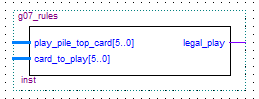
\includegraphics[scale=1.0]{rules_symb}
	\end{center}
\end{figure}
Above is a pin-out diagram of the g07\_rules circuit. A more detailed description of these ports will be given below.

\section*{Description of ports}
\addcontentsline{toc}{section}{Description of ports}

\subsection*{play\_pile\_top\_card[5..0]}
The \texttt{play\_pile\_top\_card[5..0]} is a 6 input bit vector that represents the card at the top of the play pile.
\subsection*{card\_to\_play[5..0]}
The \texttt{card\_to\_play[5.0]} is a  6 input bit vector that corresponds to the users card that they wish to play.
\subsection*{legal\_play}
The \texttt{legal\_play} output bit is active when the g07\_rules circuit determines that the input corresponds to a legal play and not active otherwise. 

\section*{VHDL charicature of the \texttt{g07\_rules} circuit}
\addcontentsline{toc}{section}{VHDL charicature of the \texttt{g07\_rules} circuit}
\label{s:vhdlrules}
The VHDL code shown below was inspired by the tactics described in the \hyperref[s:intro2]{rationale section} above.
\lstinputlisting[language=VHDL]{g07_rules.vhd}

\chapter*{With Regards to the Testing of the Rules Circuit}
\addcontentsline{toc}{chapter}{With Regards to the Testing of the Rules Circuit}
The rules of the game are very simple, since crazy eights is a game that is played by people of all
ages, and people with dementia. Here are the rules just in case the reader forgot: A card of face
value of 8 in any suit can be played on any card and can have any card played on it. Furthermore,
any card of a particular suit can be played on a card of that same suit, regardless of the cards'
values. Finally, a card with a given face value can be played on another card with the same face
value, regardless of the suits.\\\\
For any testing process to be considered legitimate, the testers must implement the appropriate
tests. Therefore, the test that were generated for this tremendous circuit were created to make sure
that every rule was tested. It was all done in the spirit of good testing. The test results may be
perused below. The returning reader may expect to find the simulation results from a Modelsim
simulation wave, however, the Modelsim simulator is simply \textit{too powerful} for such a simple
simulation. It would be innefficient to harness so much power for a circuit that doesn't require it.
Some people are less fortunate and can make use of the excess energy. So, the simulation was done
using the GTKWave VCD viewer, and is more than satisfactory for showing simple waves.

\begin{figure}[h]
	\begin{center}
		\caption{Timing simulation of the rules circuit}
		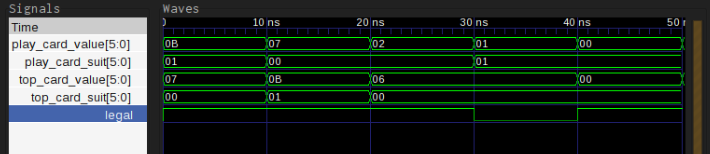
\includegraphics[scale=0.8]{rulesresults}
	\end{center}
\end{figure}

The first clock cycle is used to show that any card can be played on top of an eight, since the
eight is crazy after all. Note that the design of
the test had card values starting at 0 rather than 1, so the value of 7 for the card values actually
corresponds to a card value of 8. The second clock cycle was also used to show how crazy the eights
can be. It displayed the rule that an eight of any suit can be played over any card and due to the
design of the circuit, the test was passed. The third clock cycle was designed to make sure that a
given card of a certain suit can be played on any card of the same suit and it was an engineering
success. The penultimate clock cycle showed that a card of a given value and suit cannot be played
on another with a different value and suit, and the circuit performed like a dream. The final test
gave insight into the behavior when a card with a given face value would be played on a card with
the same face value and as stated in the rules, it was legal and did not require any additional
action to fix this violation. 

\chapter*{The Computer Analysis of the Rules Circuit}
\addcontentsline{toc}{chapter}{The Computer Analysis of the Rules Circuit}
\section*{The Flow Summary}
\addcontentsline{toc}{section}{The Flow Summary}
Quartus II’s Flow Summary reveals that the \texttt{g07\_rules} circuit uses only 46 total
combinational functions, which is quite impressive. There is a total of 18752 combinational logic
functions available in the Cyclone II DE1, thus making the total usage under 1\%. This is a
tremendous achievement because so many logic functions are left over to be used in the final design
of the great crazy eights card game. The \texttt{g07\_rules} circuit also uses zero memory bits
which is a great benefit overall. 

\section*{The Timing Analysis}
\addcontentsline{toc}{section}{The Timing Analysis}
By means of the mighty Quartus II TimeQuest Timing Analyzer, propagation delays for the two inputs
to the rules circuit were found. It was seen that the maximum propagation delay of the
\texttt{card\_to\_play} input was 19.363 nanoseconds, and the maximum propagation delay of the
\texttt{play\_pile\_top\_card} input was 19.350 nanoseconds. Therefore, the maximum propagation
delay from the input to the output is 19.363 nanoseconds. Given this propagation delay, inputs of
the system should not change more than once within a 19.363 nanosecond interval. This is reasonable
so long as the inputs of the system do not change more than once in any given interval of 19.363
nanoseconds, which is a very short amount of time.

%%%NEW CIRCUIT STARTS HERE

\part{The Dealer Circuit}

\chapter*{Introduction and Rationale}
\addcontentsline{toc}{chapter}{Introduction and Rationale}
\label{s:intro1}
As foreshadowed in the \hyperref[s:preamble]{pleasant preamble} above, having a loyal, dependable
dealer will be crucial to the reliable functionality of the crazy eights system. Without such a
dealer, the \textit{rules} of the game \textit{may not} be followed, causing complete and utter
pandemonium, ultimately resulting in a rather atrocious crazy eights game.\\\\
Therefore, it would benefit the system to create a robust \textit{finite state machine}, a machine
of a finite number of states. The system was reduced to a machine of 4 states (where $4 < \infty$
holds, proved in \hyperref[a:proof]{this appendix}), of which include the state that waits for the
previous request to end (denoted by A), the state
that waits for the next request to \textit{be} sent (denoted by B), the state that generates
random numbers, so as to deal the cards (denoted by C), and finally, the state that activates a
stack (or more accurately, a bi-directional Jenga tower) circuit (denoted by D). \\\\
All of the cleverness and power that has been teased above was encompassed by a circuit that has
since been named the \texttt{g07\_dealerFSM}. A more detailed insight to the design of the finite
state machine and the \texttt{g07\_dealerFSM} follows below, and is complemented by thoughtful
pictorial support for easier understanding.\\\\
Given the immense power of the VHDL language, implementing the state machine in code was fairly
simple. Firstly, an enumeration of states was created, and a Signal representing a state was
defined. For simplicity, it was decided to implement a Moore-type machine, meaning the output
depends only on the state of the system, held in the state signal. Then, in a \textit{process}
block, a case statement was designed, which governs state transitions based on the inputs of the FSM
and the current state of the FSM. Please enjoy the \hyperref[s:vhdl]{VHDL code} provided below for a
complete view of the dealer's design.

\chapter*{Circuit Description}
\addcontentsline{toc}{chapter}{Circuit Description}

\begin{figure}[h]
	\begin{center}
		\caption{Pin-out diagram of the \texttt{g07\_dealerFSM} circuit}
		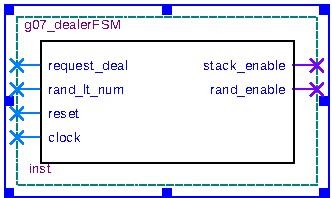
\includegraphics[scale=1.3]{dealer_symb}
	\end{center}
\end{figure}

Above is a pin-out diagram of the miraculous \texttt{g07\_dealerFSM} circuit, showcasing its input
and output ports. A more detailed description of these ports will be given below.

\section*{Description of ports}
\addcontentsline{toc}{section}{Description of ports}
\subsection*{request\_deal}
The \texttt{request\_deal} input bit is activated when the system requests that the dealer should
deal a card.
\subsection*{rand\_lt\_num}
The \texttt{rand\_lt\_num} input bit is controlled by an external circuit that is high when a random
number has a value that is less than the BJT's \texttt{NUM} output that the dealer is associated
with. This allows the dealer to tell whether it should keep generating random numbers (in state C),
or move on.
\subsection*{reset}
The \texttt{reset} input bit causes the finite state machine to be reset to its initial state when
\texttt{reset} is high. It is asynchronous.
\subsection*{stack\_enable}
The \texttt{stack\_enable} output bit is active when a valid random number has been generated in the
proper state. It is used to enable the BJT associated with the dealer to pop a card.
\subsection*{rand\_enable}
The \texttt{rand\_enable} output bit is active after \texttt{request\_deal} has been asserted anew,
and enables a random number generator to generate random numbers until \texttt{rand\_lt\_num} is
high.\\\\

A complete VHDL description of the \texttt{g07\_dealerFSM} circuit is provided in the following
section.

\section*{VHDL portrayal of the \texttt{g07\_dealerFSM} circuit}
\addcontentsline{toc}{section}{VHDL portrayal of the \texttt{g07\_dealerFSM} circuit}
\label{s:vhdl}
The tactics used to develop this VHDL code may be examined in the \hyperref[s:intro1]{rationale
section} above.
\lstinputlisting[language=VHDL,breaklines=true,frame=single]{g07_dealerFSM.vhd}

\chapter*{On the Testing of the Dealer Circuit}
\addcontentsline{toc}{chapter}{On the Testing of the Dealer Circuit}
It was an important and difficult challenge to resist being seduced by the beauty of the VHDL code
that describes the \texttt{g07\_dealerFSM} circuit. Despite it's beauty, a dealer cannot be trusted
without being tested. Think about this following section as an analog to an interview process, if
you will. Before putting the \texttt{g07\_dealerFSM} in commission, it was important to make sure it
satisfied all dealing requirements (and boy, did it ever), and to make sure it functioned correctly
on the hardware. The demonstrations that follow will prove that the \texttt{g07\_dealerFSM} is in
fact an excellent candidate.

\section*{The software circuit simulation: a poor man's analysis}
\addcontentsline{toc}{section}{The software circuit simulation: a poor man's analysis}
The first order of business in judging the effectiveness of the \texttt{g07\_dealerFSM} was to test
it with the magical Modelsim simulator. Unfortunately, said software was not functioning to the
tester's standards. As a consequence, the miraculous GtkWave VCD viewer came to the rescue, and the
\texttt{g07\_dealerFSM} was examined thoroughly according to a
\hyperref[a:dealertst]{carefully-written testbench}. \\For the less-enthused, the testbench starts the
state machine in its default state, and examines each state transition in the trivial order. Then,
the machine is brought to state C (where \texttt{rand\_enable} is high) and reset is activated to
ensure that it causes the machine to return to its initial state.\\
The resulting waveforms can be viewed below.\\\\
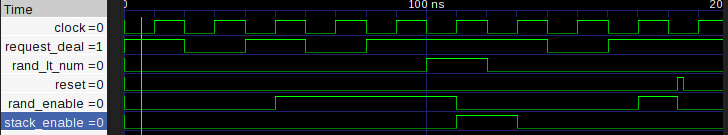
\includegraphics[scale=0.75]{dealertestcropped}
Of course, the results shown above cannot conclusively confirm the excellence of the
\texttt{g07\_dealerFSM} circuit on their own, because they give no evidence of the dealer
functioning on real hardware. Hence, this test was called a \textit{poor man's
analysis}. Fortunately, the testers \textit{are not} poor men. In fact, they have access to an
Altera DE1 FPGA development board equipped with an Altera Cyclone II FPGA. The tests in the
following section will describe how \textit{full confidence} of the \texttt{g07\_dealerFSM} was
obtained.

\section*{The hardware circuit simulation: an Engineer's victory}
\addcontentsline{toc}{section}{The hardware circuit simulation: an Engineer's victory}
Some tests are easy, leaving the participants in a relaxing state of mind. Yet, some tests are hard,
leaving participants in a state of panic. However, occasionally a test may reach a transcendental level of
difficulty, such that it may be said that the test \textit{separates the boys from the men}. That,
dear reader, is what you will witness in the remainder of this section. Anyone from laymen to
patricians can make a software circuit simulation, neglecting the possiblity that something may go
wrong on the hardware. While seemingly reasonable to the un-seasoned tester, this train of thought
is highly dangerous and irresponsible. It is up to the Engineer to realize that this, in fact, will
not suffice. This realization was exhibited, more than anything else, in the results below. \\\\
The first order of business was to create a \textit{test bed}, or circuit that bridges the gap
between human input and dealer communication. This was done using the not-short-of-incredible Altera
Quartus II schematic designer, and may be perused \hyperref[a:testbed]{here}.\\\\
For the less-motivated reader, a brief description of the testbed will be given. Firstly, The
\texttt{stack\_enable} output of the dealer circuit is passed as the \texttt{enable} input of the
BJT. The \texttt{rand\_enable} output was passed to the \texttt{enable} input of a
\texttt{g07\_register6} circuit, which is a masterfully-simple 6-bit register designed by the same
designers of the \texttt{g07\_dealerFSM}. The design of the \texttt{g07\_register6} is unfortunately
beyond the scope of this report. The register serves the purpose of latching a random
number generated by the random number generator module. Then, the value stored by the register is
passed through a comparator, which sends a 1 to the \texttt{g07\_dealerFSM} when the random value is
less than the \texttt{NUM} output of the BJT. The \texttt{request\_deal} input comes from the output
of the infamous \texttt{g07\_debounder} debouncer circuit (discussed in a previous laboratory
report), so as to remove the all-feared bouncing of the DE1's hardware buttons. The random number
generator module consists
of a \texttt{g07\_RANDU} (discussed in a previous laboratory report) which takes as input the
multiplexation of a constant seed, and the last generated random output of itself. When the BJT is
full, the constant seed is passed to the RANDU, and otherwise it uses its own seed to enliven
itself.\\\\
Finally, the \texttt{NUM} output of the BJT as well as the \texttt{VALUE} output corresponding to
the address described by the value stored in the \texttt{g07\_register6} are passed through
\texttt{mod13} circuits (discussed in previous laboratory reports) to be conveniently displayed on
the 7 segment decoders on the DE1 board.\\\\
Some say a picture is worth a thousand words, however only an infinite amount of words can be used
to describe the joy of the testers upon witnessing the massive success of the
\texttt{g07\_dealerFSM} circuit on the testbed. It would be infeasible to include so many pictures
in this report. Instead, a brief overview of what was accomplished will be offered.\\\\
There were just two more criteria that needed to be confirmed to ensure the proper functioning of
the dealer. Firstly, it needed to be confirmed that the \texttt{NUM} output of the BJT decreases by
only 1 after each deal (thus implying that the dealer deals one card at a time). This test passed
immediately with flying carpets. Furthermore, it had to be ensured that the cards being dealt were
random! Although this part did provide some inconsistencies early one (due to a mistake with the
comparator connections, mostly), eventually it was seen that random numbers in the range of 0 to
\texttt{NUM} were seen being popped from the BJT. Victory was gracefully achieved.

\chapter*{Computer Analysis of the Dealer Circuit}
\addcontentsline{toc}{chapter}{Computer Analysis of the Dealer Circuit}
If you thought the validation of the \texttt{g07\_dealerFSM} circuit was complete, you have
successfully been tricked. What blasphemy! Surely, the \texttt{g07\_dealerFSM} must be shown to not inhibit the
circuitry that it will integrated with. To verify that this will not be an issue, Altera's magical
Quartus II Flow Summary and TimeQuest Timing Analyzer will be used extensively. Please continue
reading the final sections of this report to determine whether or not the \texttt{g07\_dealerFSM} is
a \textit{feasible} circuit, given all its unwieldly power.

\section*{The Flow Summary}
\addcontentsline{toc}{section}{The Flow Summary}
According to Quartus II's Flow Summary, the \texttt{g07\_dealerFSM} allegedly uses only 3
combinational logic functions, and 3 dedicated logic registers. Given that there are 18752 logic
registers and combinational logic functions available in the FPGA, these numbers make for less than
1\% of the resources available. Then, it can be safely concluded that the \texttt{g07\_dealerFSM}
does not require too much hardware, and is in fact \textit{very} feasible in that regard.
Furthermore, the \texttt{g07\_dealerFSM} allegedly requires absolutely no memory bits, further
convincing the feasibility of the dealer.

\section*{The Timing Analysis}
\addcontentsline{toc}{section}{The Timing Analysis}
Lastly (and you are not being fooled this time), the dealer must not require particularly low clock
frequencies for its operation to be successful. It also would be beneficial for it to not impose any
restrictions on the envelope of the clock pulse, as that would be rather inconvenient. According to
the Timing Analyzer of Quartus II, the \texttt{g07\_dealerFSM} allegedly imposes a minimum pulse
width of -1.631 nanoseconds. Negative pulse widths are not a problem
in the measuring systems in use today. In fact, most may say negative pulse widths do not exist (but
it's better not to generalize in a report like this). However, due to the negative minimum pulse
width, it can be safely concluded that no testable pulse width should cause a problem for the
\texttt{g07\_dealerFSM} circuit.\\\\
Finally, the Quartus II Timing Analyzer reported a restricted maximum frequency of 380.08MHz. This
is extremely impressive, given that the maximum clock frequency that will be supplied to the
\texttt{g07\_dealerFSM} is the DE1's clock of 50MHz. Therefore, there shall be no timing violations
caused by the \texttt{g07\_dealerFSM} given its clock. This maximum frequency corresponds to a
maximum propagation delay within the circuit of $1/38008000 = 2.63$ns, which is exceedingly
small.\\\\
Given these results, it is clear that the \texttt{g07\_dealer} circuit uses very little hardware and
imposes no considerable timing issues. Finally, the Engineer may leave his mark.
\begin{appendix}
	\chapter{VHDL Testbench for the \texttt{g07\_dealerFSM}}
	\label{a:dealertst}
	\lstinputlisting[language=VHDL]{dealerFSM_tst.vhd}
	\chapter{Testbed for the \texttt{g07\_dealerFSM}}
	\label{a:testbed}
	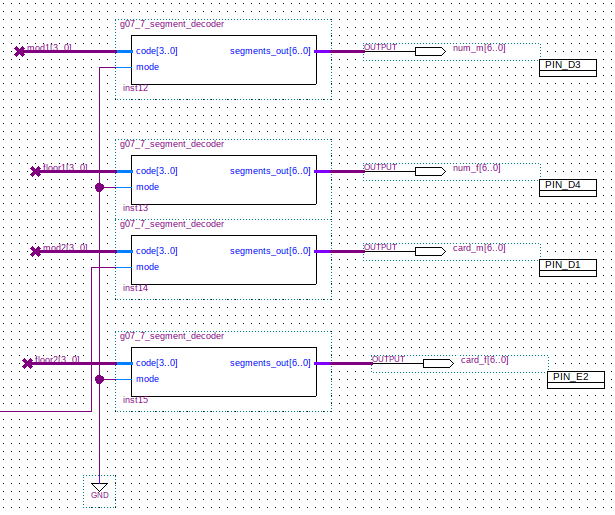
\includegraphics[scale=0.8,angle=0]{testbed_led}\\
	Above is the section of the testbed that showws how data is output to the 7 segment displays on
	the DE1. On the following page, the main body of the testbed may be observed.
	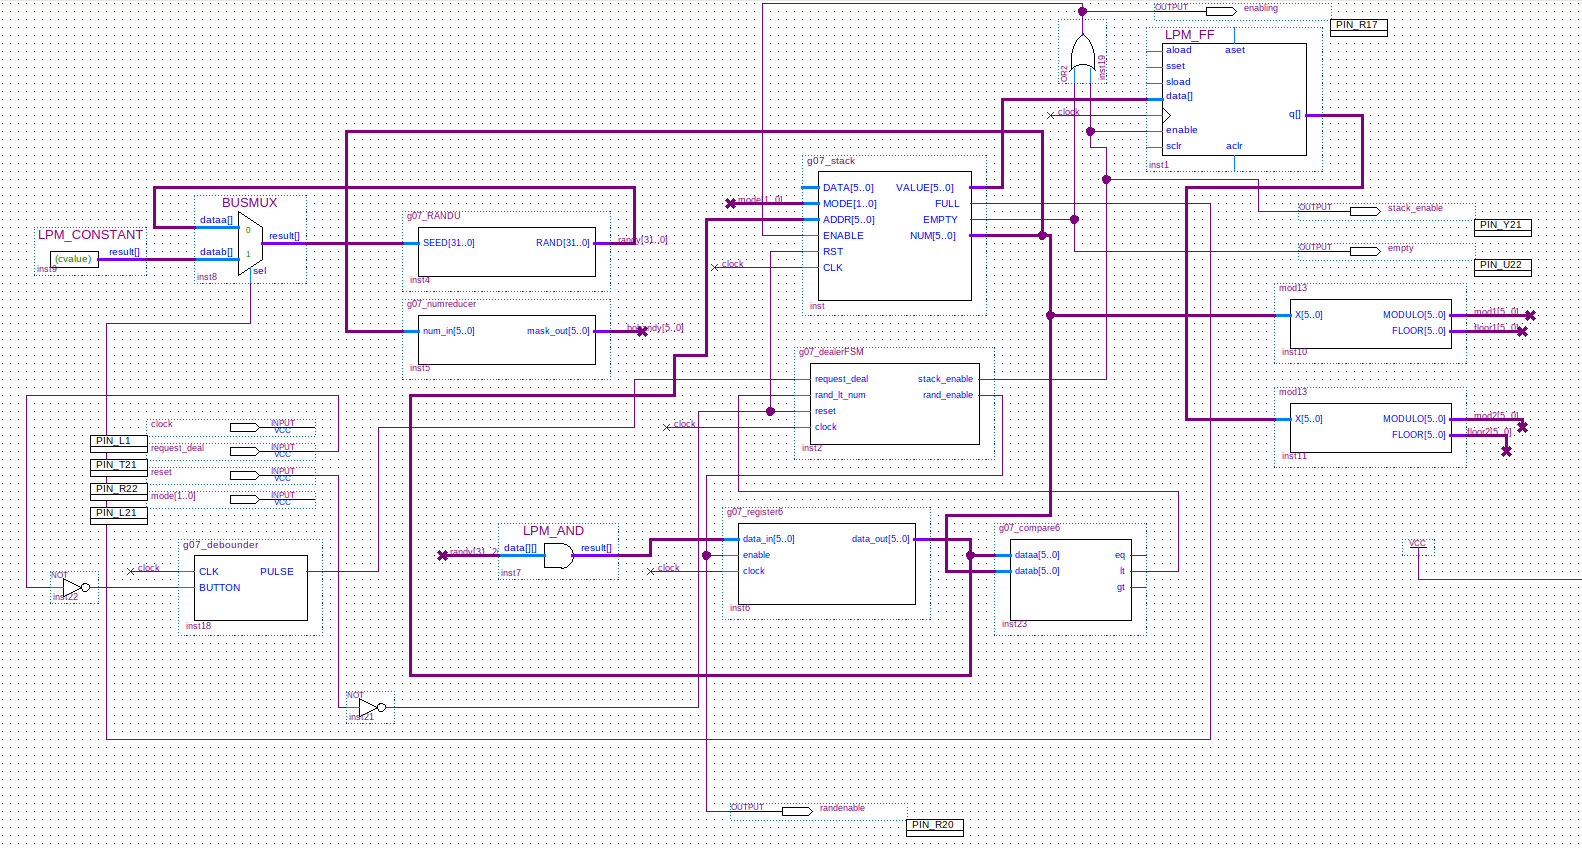
\includegraphics[scale=0.5,angle=270]{testbed_body}
	\chapter{Proving the Finite-ness of the State Machine}
	For the precise reader, stating that the desgined state machine is actually finite may not be
	concrete enough to be taken seriously. Given that the amount of states in the machine is 4, it
	can be shown that the machine is in fact finite.\\\\
	\textbf{Proof:} $4 < \infty$\\
	\label{a:proof}
	Follow a proof by contradiction.
	Assume $4 \geq \infty$. Then, 
	\begin{equation*}
		\begin{aligned}
			\sum_{k=0}^{\infty}x^k &\leq \infty, \ |x| < 1\\
			10\sum_{k=0}^{\infty}x^k &\leq \infty\\
			10\sum_{k=0}^{\infty}x^k &\leq 4\\
		\end{aligned}
	\end{equation*}
	Choose $x = \frac{1}{2}$. It can be shown combinatorially that $\frac{1}{2} < 1$ as follows:
	suppose two individuals are sharing a cake. By definition, the amount of cake each individual
	can eat is $\frac{1}{2}$ of the cake. Since energy can neither be created or destroyed, the
	amount of cake cannot be increased when two people share it. Thus, $\frac{1}{2} < 1$.\\\\
	\textbf{Corollary 1:} $\frac{1}{2} < 1$. \\
	Binding $x$ to $\frac{1}{2}$, the following can be discovered:
	\begin{equation*}
		\begin{aligned}
			10\sum_{n=0}^{\infty}\frac{1}{2}^k &\leq 4\\
			10\left(1 + \frac{1}{2} +\frac{1}{4} + \frac{1}{8} + \frac{1}{16} + \dots\right) &\leq 4\\
			10\left(1 + \aleph\right) &\leq 4, \ \aleph > 0\\
			10 + 10\aleph &\leq 4 \rightarrow 10\aleph \leq -6
%			10\aleph &\leq -6
		\end{aligned}
	\end{equation*}
	Clearly, this is a contradiction since the definition of $\aleph$ guarantees that it is
	positive.\\
	Therefore, by contradiction, $4 < \infty$.

\end{appendix}

\end{document}
